\chapter{Image Denoising}

\section{An ill-posed problem}
\begin{itemize}
\item It is not possible to separate the original (noise-free) image
  from noise \cite{wikipedia_ill_posed_problem}.
\item But there are ad-hoc
    solutions \cite{wikipedia_noise_reduction}.
\end{itemize}

\section{Thermal noise}
\begin{itemize}
\item Significative in \gls{MRI}.
\item Originated by the thermal motion of the atoms and therefore, of
  the electrons.
\item Described as a grainy, random texture.
\item Modeled as additive Gaussian noise or, in the case of \gls{MRI}
  as additive Rician noise \cite{wikipedia_Rice_distribution}, because
  the noise is captured in the frequency domain.
\end{itemize}

\section{Quantum mottle (quantum noise)}
\begin{itemize}
\item Appears in X-ray and \gls{CT} images.
\item Consequence of the \popup{small number
    of photons}{Remember that the radiation must be minimized and the
    number of X-ray photons is proportional to the energy of the
    radiation.} that reach the detector.
\item Looks like grainy noise. 
\item Mathematically modeled as a \popup{(multiplicative)}{By
    definition, Poisson noise is multiplicative.} Poisson
  distribution \cite{wikipedia_Poisson_distribution}.
\end{itemize}

\section{Speckle (interference) noise}
\begin{itemize}
\item Significative in low-SNR areas of \gls{MRI} images and in ultrasound images.
\item Generated by the constructive and destructive interference of
  \popup{coherent waves}{Waves are in phase.}, such as laser light or
  radar waves, interacting with a target.
\item Described as granular, textured pattern.
\item Usually modeled as multiplicative Gamma distribution (or more
  specifically, a Rayleigh distribution
  \cite{wikipedia_Rayleigh_distribution} for the signal amplitude).
\end{itemize}

\section{Physiological noise \cite{scarciglia2023physiological}}
\begin{itemize}
\item Significative in \gls{MRI}, and it is independent of $B_0$ (the
  strength of the magnetic field).
\item Refers to undesired signal variations caused by the patient's
  own bodily functions, primarily cardiac (heartbeat) and respiratory
  (breathing) cycles. These processes induce changes in cerebral blood
  flow, blood volume, and cerebrospinal fluid flow, generating
  magnetic field fluctuations.
\item Non uniform (depends on the scanned area) and difficult to model.
\end{itemize}

\section{Denoising \cite{buades2005review}}
\begin{itemize}
\item Denoising (the removal of the noise) is carried out in
  medical imaging to improve the \gls{SNR}, with the ultimate
  objective of increase the accuracy of the diagnoses.
\item Unfortunately, it is difficult to remove only noise (some part
  of the signal, typically the high frequency components of the signal
  are also filtered-out.
\end{itemize}

\section{Gaussian filtering \cite{gonzalez2009digital}}
\begin{itemize}
\item Spatial (2D) filter \popup{using 1D Gaussian}{The filter is
  separable, which means that the image can be filtered by rows and
  columns, using always 1D kernels.} \popup{kernels}{Filter is
  another name for the filter structure.}.
\end{itemize}

\begin{figure}[H]
  \vspace{-1ex}
  \centering
  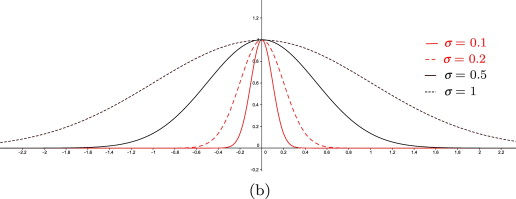
\includegraphics[width=0.8\textwidth]{Gaussian_kernels}
  \caption[The Gaussian kernel.]{Function that determines the
    coefficients of a Gaussian kernel. $\sigma$ \popup{controls the
      bandwidth}{Bandwidth decreases with increasing sigma.} of the
    Gaussian \popup{filter}{That is a low-pass filter.}.}
  \label{fig:gaussian_kernel}
\end{figure}

\begin{itemize}
\item Isotropic (it \popup{blurs pixel values equally in all directions}{Which
  softens noise but also destroys important edges.}).
\end{itemize}

\begin{figure}[H]
  \vspace{-0ex}
  \centering
  \href{https://www.cloudfactory.com/blog/gaussian-noise-medical-ai}{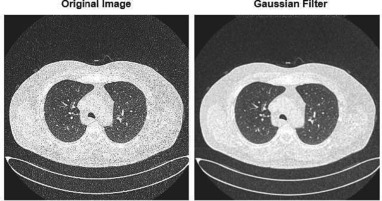
\includegraphics[width=0.9\textwidth]{GF_example}}
  \caption{Gaussian denoising example.}
  \label{fig:gaussian_denoising_example}
\end{figure}

\section{\glsentrylong{AND} (\glsentryshort{AND}) \cite{gonzalez2009digital}}
\begin{itemize}
\item Anisotropic (only blurs in the direction of the minimum
  gradient, i.e., the edged are preserved).
\end{itemize}

\begin{figure}[H]
  \vspace{-0ex}
  \centering
  \href{https://dsp.stackexchange.com/questions/14606/anisotropic-diffusion}{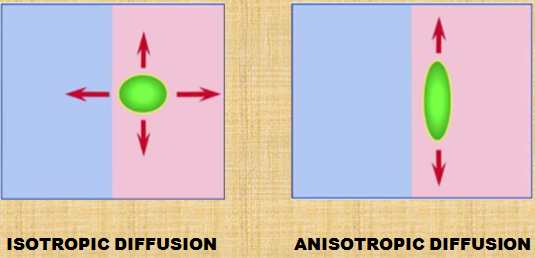
\includegraphics[width=10cm]{anisotropic_diffusion}}
  \caption[Isotropic VS anisotropic filtering.]{Isotropic VS
    anisotropic filtering. The kernel is longer in the direction of
    the edge.}
  \label{fig:AND_filtering}
\end{figure}

\begin{figure}[H]
  \vspace{-0ex}
  \centering
    \href{https://es.mathworks.com/help/images/ref/imdiffusefilt.html}{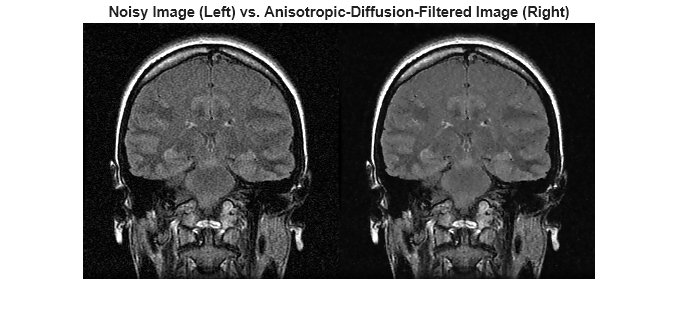
\includegraphics[width=\textwidth]{AD_example}}
  \caption{\gls{AND} denoising example.}
  \label{fig:AND_denoising_example}
\end{figure}

\section{Wiener denoising \cite{gonzalez2009digital}}
% Include also filtering in the wavelet domain because can be useful for removing specke noise.
\begin{itemize}
\item Wiener developed an adaptive filter based on a predictor capable
  of restore the \popup{image}{A signal in general.} in several
  aspects, for example,
  \href{https://docs.opencv.org/3.4/d1/dfd/tutorial_motion_deblur_filter.html}{to
    correct the blur generated by motion}.
  \begin{figure}[H]
    \vspace{2ex}
    \centering
    \href{https://docs.opencv.org/3.4/white_car.jpg}{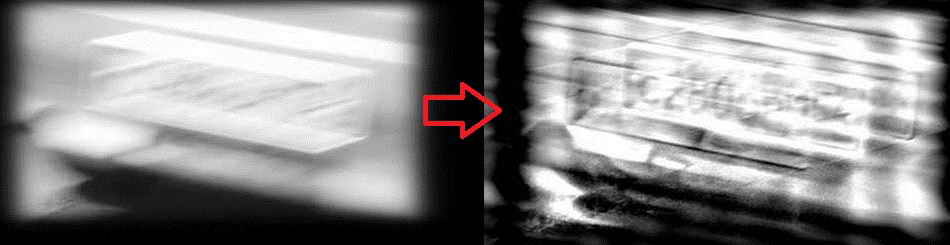
\includegraphics[width=\textwidth]{wiener_deconvolution}}
    \caption{A motion deblur example using Wiener deconvolution.}
    \label{fig:Motion_deblur}
  \end{figure}
\end{itemize}

\begin{itemize}
\item Using a Wiener filter we can also \popup{remove}{The correct
    word here (and in all the denoising techniques) should be
    ``minimize''. Only if the noise signal were known, the original
    (clean) signal could be completely restored.} \popup{additive
    noise}{A random signal that has been added to the clean signal,
    and that is independent of the clean signal.} of a image by
  estimating the amplitude of the noise. The idea is to use a
  \popup{bluring filter}{A low-pass filter, such as a Gaussian kernel}
  \popup{adapted to the energy of the noise}{The higher the amplitude
    of the noise, the longer the kernel, i.e., the higher the blur
    effect, and therefore, the higher the noise removal.} \popup{in
    each area}{For this reason, one of the parameters of the Wiener
    filter for denoising is the size of a square window.} of the
  image.
  \begin{figure}[H]
    \vspace{2ex}
    \centering
    \href{https://www.techscience.com/csse/v45n2/50440/html}{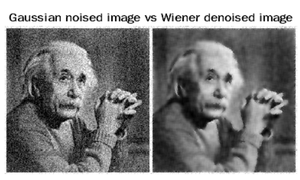
\includegraphics[width=8cm]{wiener_albert}}
    \caption{Removal of Gaussian noise using Wiener denoising.}
    \label{fig:Wiener_denoising}
  \end{figure}
\end{itemize}

\section{\gls{NLM} \cite{buades2010image}}
\begin{itemize}
\item Most images are redundant in terms of the different local
  textures and patterns that define them.
  \begin{figure}[H]
    \vspace{2ex}
    \centering
    \href{https://docs.opencv.org/3.4/d5/d69/tutorial_py_non_local_means.html}{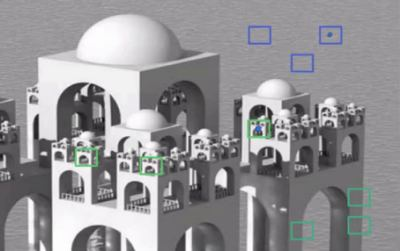
\includegraphics[width=8cm]{NLM_opencv}}
    \caption{Example of patch selection in \gls{NLM}.}
    \label{fig:NLM_patching}
  \end{figure}
\end{itemize}
  
\begin{itemize}
\item The mean of the noise \popup{is usually zero}{And if the mean
  ins not zero, we can substract the mean of the noise.}, i.e.,
  the average of different instances of the same signal tends to the
  clean signal logarithmically.
  \begin{figure}[H]
    \vspace{0ex}
    \centering
    \href{https://www.umbjournal.org/article/S0301-5629(17)30201-6/fulltext}{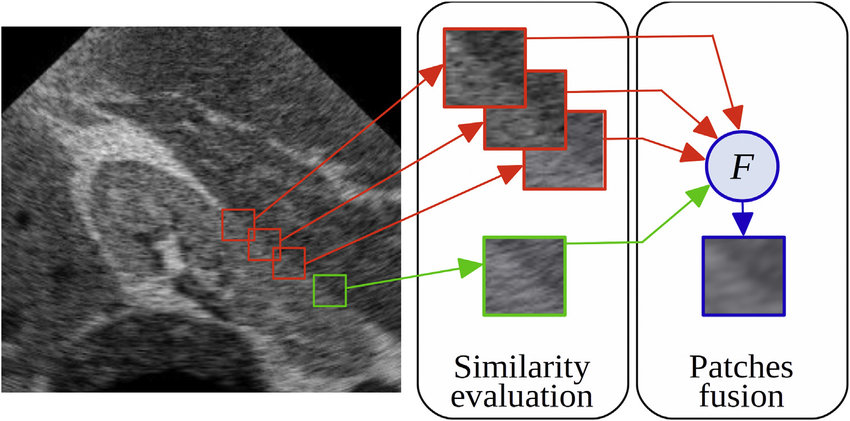
\includegraphics[width=10cm]{NLM_example}}
    \caption{\gls{NLM} patches averaring.}
    \label{fig:NLM_averaging}
  \end{figure}
\end{itemize}

\begin{figure}[H]
  \vspace{0ex}
  \centering
  \begin{tabular}{cc}
    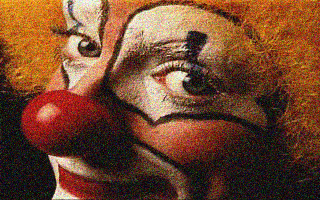
\includegraphics[width=6cm]{clown-noise-25} & 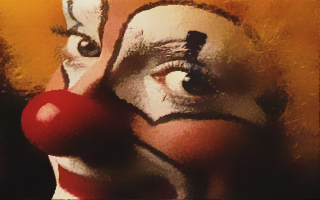
\includegraphics[width=6cm]{NLM_clown}
  \end{tabular}
  \caption{A \gls{NLM} filtering \href{https://imagej.net/plugins/non-local-means-denoise/}{example}.}
  \label{fig:NLM_example}
\end{figure}

\section{U-Net denoising}
\begin{itemize}
\item An U-Net denoiser is an \popup{\gls{ANN}}{An ANN is a
  computational structure that is inspired in the real neurons of
  the brain, and how they interact. ANNs is only a type of this
  kind of structures. In a more global context of machine, we use
  the word ``model'' to refer to the structure.} trained for the
  removal of noise in images.
\item Training is an iterative process, where a
  \popup{collection}{In general, very large (millions).} of
  \popup{convolutional neurons}{The word convolution comes from the
    name of the mathematical operation (convolution) that in the
    context of signal processing describes a filtering process.}
  (organized in 2D \popup{layers}{Convolutional layers.}) optimize
  the weights of their interconnections to transform an input into a
  \popup{desired}{In general, only approximated.} output. In the
    case of an U-Net for denoising, in each iteration, at the input we
    put a noisy \popup{image}{When, during the learning, we input to
      the model the raw data (instead of a preprocesed version of it)
      we use the concept of deep learing.}, and at the output the
    corresponding clean image.
\end{itemize}
\begin{itemize}
  \item Therefore, an U-Net can be defined as a
    \popup{feed-forward}{The data flows fron the input to the output
      without loops.} \popup{\gls{CNN}}{In a CNN, the convolutional
      neurons of the i-th layer only are directly connected a limited
      number of neurons of the (i+1)-th layer: those neurons that are
      spatially close. We we deal with images, we organize the neurons
      by small square reguions. The size of these regions define the
      size of the 2D kernels used for the filtering process. During
      the learning, for an output channel, the neurons of a layer
      found those filtering coefficients (weights) that allow to
      approximate the input to the output. All the neurons of this
      layer use the same kernel (share the same weights), for a given
      output channel. Notice that in the following example only one
      output channel per convolutional layer has been used. In
      general, at least in an U-Net, we work with several (dozens of)
      channels.}.
\end{itemize}

\begin{figure}[H]
  \vspace{0ex}
  \centering
  \href{https://en.wikipedia.org/wiki/Convolutional_neural_network#/media/File:1D_Convolutional_Neural_Network_feed_forward_example.png}{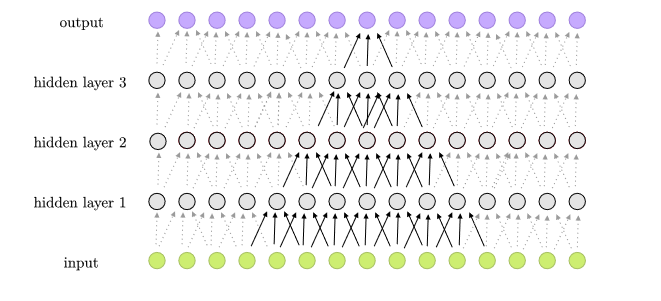
\includegraphics[width=8cm]{1D_Convolutional_Neural_Network_feed_forward_example}}
  \caption{A 1D \gls{CNN} where the connection degree (kernel size) is 3.}
  \label{fig:a_CNN}
\end{figure}

\begin{itemize}
\item Using
  \href{https://en.wikipedia.org/wiki/Backpropagation}{back-propagation}
  the neurons learn which must be the weights between them to
  minimize the \popup{error}{Some definition of the error, for
    example, the MSE.} between the input and the output. In our
  case, the \popup{error}{The difference between the input and the
    output.} is the noisy image. Therefore, the neurons learn how to
  get rid of the noise.
\item Therefore, in a U-Net denoiser, the popup{output}{Of the last
  layer.} \popup{feature map}{The 2D array (image) with the
  output of each neuron in a channel.} is the denoised image.
\item
  \href{https://github.com/vicente-gonzalez-ruiz/medical_imaging/blob/main/notebooks/U_Net.ipynb}{Here}
  you have a toy example of an U-Net that can help to understand all
  these concepts and the potential of the \gls{AI}-based denoising
  techniques.
\end{itemize}

\begin{itemize}
\item U-shaped.
\end{itemize}

\begin{figure}[H]
  \vspace{0ex}
  \centering
      \href{https://www.linkedin.com/pulse/14-coding-u-net-architecture-from-scratch-riya-chhikara-xbvte}{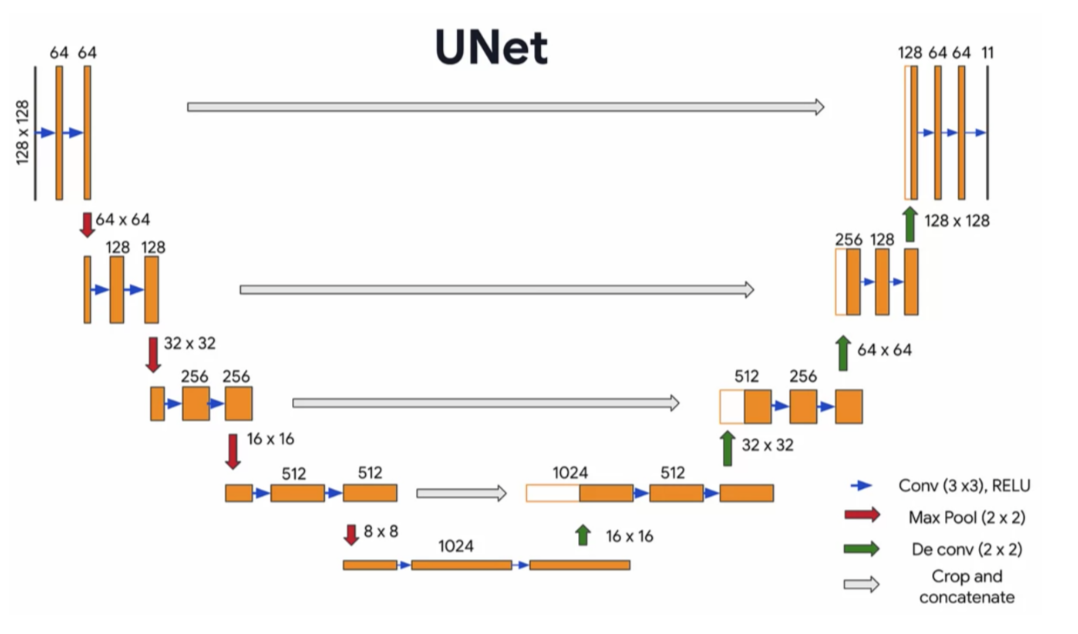
\includegraphics[width=12cm]{U-Net}}
  \caption{Example of the architecture of an U-Net for patches of $128\times 128$.}
  \label{fig:UNet}
\end{figure}

\begin{itemize}
\item Patching.
\end{itemize}

\begin{figure}[H]
  \vspace{0ex}
  \centering
  \href{https://www.linkedin.com/pulse/attention-guided-u-net-model-improved-residual-blocks-gokmen}{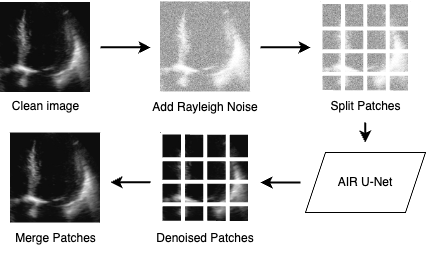
\includegraphics[width=10cm]{U-Net_example}}
  \caption[Patching with an U-Net.]{Filtering of a image with more resolution than the U-Net input using patches.}
  \label{fig:patching}
\end{figure}
